\chapter{Korisničko uputstvo}
\begin{enumerate}
    \item \textbf{Uspostavite internet konekciju} prema uputama vašeg instruktora.
    \begin{enumerate}
        \item potrebno je da na mreži bude dostupna Logit serverska aplikacija i certifikacijski repozitorij za uspješnu prijavu i korištenje, dostupnost možete provjeriti posjetom na \url{https://logit.mine.nu:5000}
    \end{enumerate}
    \item \textbf{Uključite lokacijske usluge} vašeg Android mobilnog uređaja.
    \begin{enumerate}
        \item detaljno uputstvo možete pronaći na \url{https://support.google.com/accounts/answer/3467281?hl=hr}
    \end{enumerate}
    \item \textbf{Omogućite NFC komunikaciju} na vašem Android mobilnom uređaju i \textbf{isključite Android Beam} uslugu za optimalan rad aplikacije.
    \begin{enumerate}
        \item \texttt{Settings > NFC > Enable}
        \item \texttt{Settings > NFC > Android Beam > Disable}
        \item više detalja za navedene postavke pročitajte na \url{https://support.google.com/nexus/answer/2781895?hl=hr}
    \end{enumerate}
    \item Ukoliko niste, \textbf{omogućite sigurnosnu funkcionalnost zaključavanja vašeg ekrana}
    \begin{enumerate}
        \item Android OS nudi usluge integrisane sigurnosti mobilnih uređaja, te je Keystore funkcionalnost sigurnog pohranjivanja privatnih ključeva usko vezana za ostale sigurnostne postavke, stoga omogućite zaključavanje ekrana slijedeći uputstvo na \url{https://support.google.com/nexus/answer/2819522?hl=hr}
    \end{enumerate}
    \item Prihvatite poziv za alpha testiranje posjetom na \url{https://play.google.com/apps/testing/ba.unsa.etf.logit} i nastavite na Play Store te \textbf{instalirajte aplikaciju}
    \begin{enumerate}
        \item ukoliko vaš mobilni uređaj nije izlistan kao podržan obratite se vašem instruktoru i biti će vam izdat jedinstveni NFC Certifikat, koji ćete koristiti za bilježenje prisustva
    \end{enumerate}
    \item \textbf{Pokrenite Logit aplikaciju}
    \item \textbf{Unesite vaše ZAMGER korisničke podatke}, ovi podatci koriste se jednokratno za provjeru valjanosti identiteta prije generisanja vašeg para ključeva, vaša lozinka ne ostaje pohranjena na Logit sistem i prenosi se https kanalom prema ZAMGER servisu
    \item Aplikacija je spremna za korištenje i ne mora biti pokrenuta u prednjem planu za prijavu prisustva, \textbf{za optimalne rezultate} dovoljno je da upalite ekran vašeg Android uređaja na “lock screen” i prislonite na Android uređaj instruktora.
    \item \textbf{Ukoliko želite koristiti aplikaciju u instruktorskom modu} i prikupljati prisustvo, dovoljno je da pokrenete Logit aplikaciju u prednjem planu te prislonite vaš uređaju studentskom uređaju u skladu sa korakom 8.
\end{enumerate}

\pagebreak[4]
\section{Instruktorski način rada}
\paragraph*{}
Pokretanjem glavnog prozora Logit aplikacije ulazite u mod za prikupljanje studentskih potpisa prisustva. Ovaj zaslon podijeljen je na četiri komponente, opisi kako slijedi u nastavku.

\begin{figure}[H]
    \centering
    
\includegraphics[width=0.6\textwidth]{material/manual/01-head}
    \caption{Zglavlje aplikacije prikazuje aktivnog korisnika}
\end{figure}

\begin{figure}[H]
    \centering
    
\includegraphics[width=0.6\textwidth]{material/manual/02-menu}
    \caption{Glavni izbornik, opisi funkcionalnosti u nastavku}
\end{figure}

\begin{description}[noitemsep,align=right,labelwidth=2cm]
    \item [Dugme 1] služi za ručno osvježavanje trenutne lokacije
    \item [Dugme 2] koristite za provjeru valjanosti ključeva korištenih pri potpisu
    \item [Dugme 3] sinhronizacija trenutne sesije na Logit server, svi potpisi se pohranjuju u jednu sesijsku cjelinu i brišu sa mobilnog uređaja (kreira se nova sesija)
    \item [Dugme 4] otvara e-mail klijent po izboru korisnika u cilju lakše prijave grešaka
\end{description}

\begin{figure}[H]
    \centering
    
\includegraphics[width=0.6\textwidth]{material/manual/03-geobar}
    \caption{Trenutno zabilježena lokacija korisničkog uređaja}
\end{figure}

\begin{figure}[H]
    \centering
    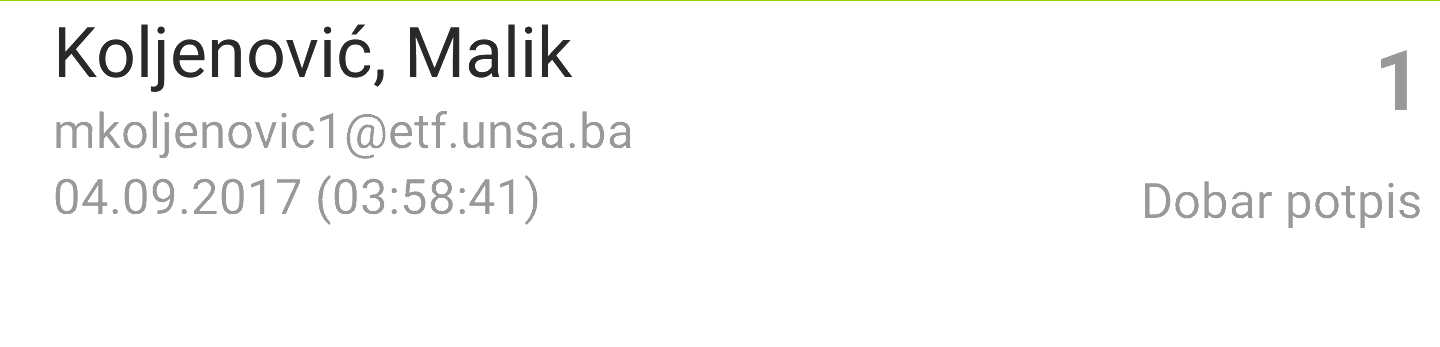
\includegraphics[width=0.6\textwidth]{material/manual/04-attns}
    \caption{Ordinalno numerisan spisak prisutnih studenata}
\end{figure}